\documentclass{beamer}
\usepackage[english,russian]{babel}
\usepackage[utf8]{inputenc}
\usepackage{amsmath}
\usepackage{hyperref}
\usetheme{Warsaw}
\usepackage{listings}
\usepackage{xcolor}
\usepackage{tikz}
\usetikzlibrary{graphs}
\usepackage{algpseudocode}

\lstset{
    frame=tb,
    tabsize=4,
    showstringspaces=false,
    numbers=left,
    commentstyle=\color{green},
    keywordstyle=\color{blue},
    stringstyle=\color{red},
    emph={baz},
    emphstyle=\textbf
}

\begin{document}

\title{SAT/SMT solvers\newline  1. Arrays}
\author{Roman Kholin}
\institute{Lalambda}
\date{Tbilisi, 2023}

\begin{frame}
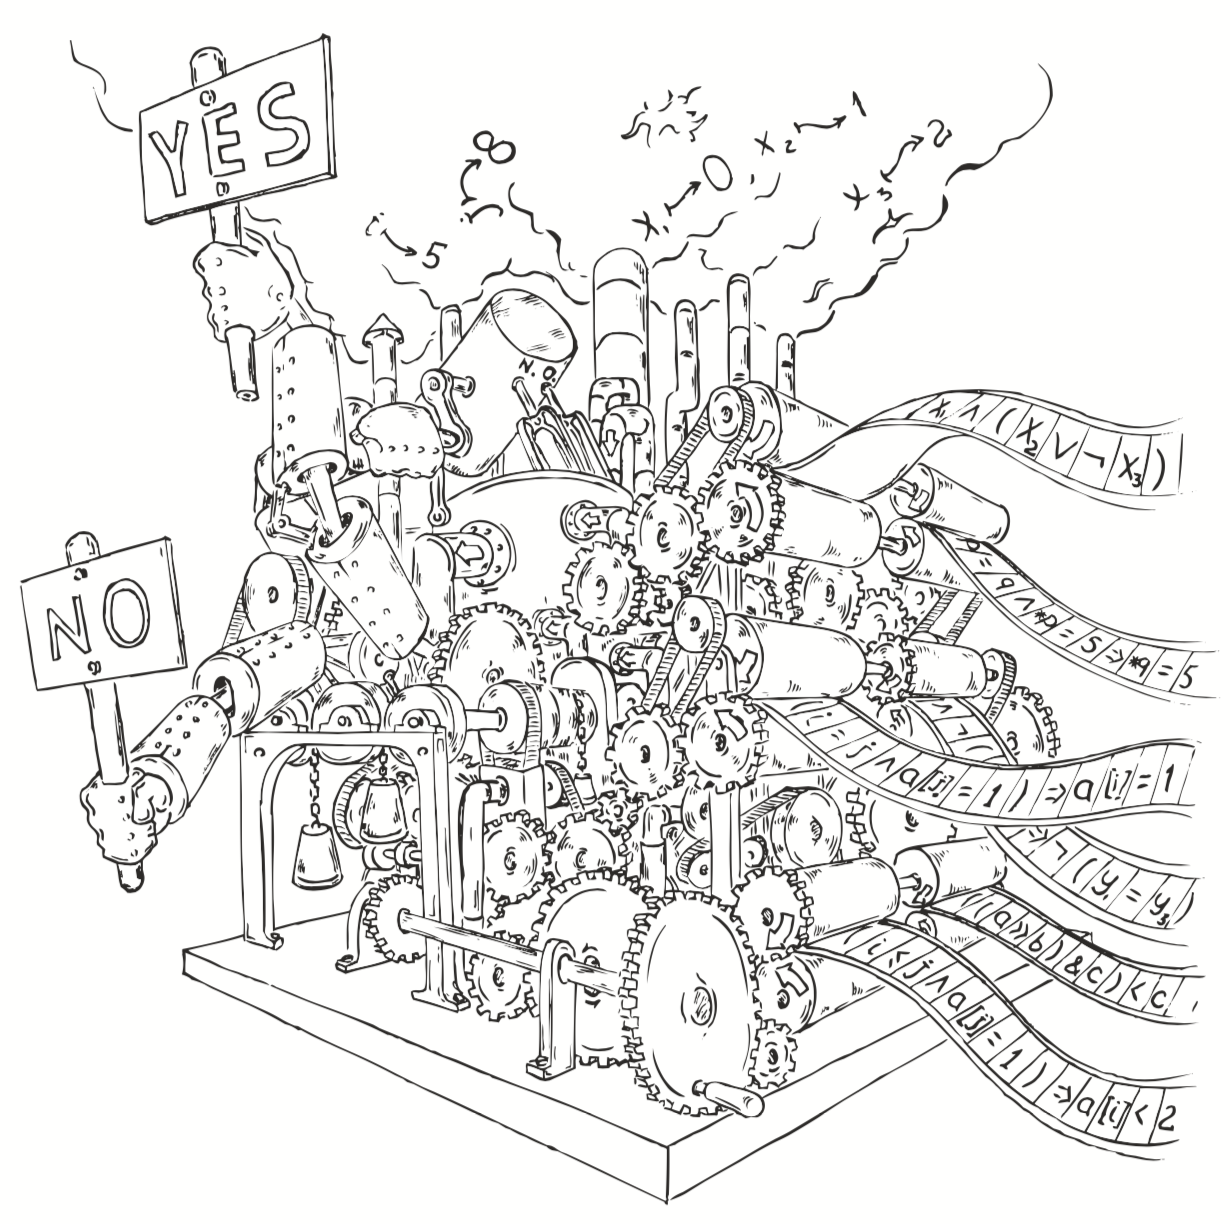
\includegraphics[scale=0.5]{../decision-procedure.png}
\end{frame}

\frame{\titlepage}

\begin{frame}{Example}
Verification conditions:\newline
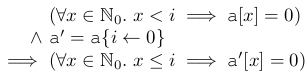
\includegraphics[scale=0.5]{conditions.png}
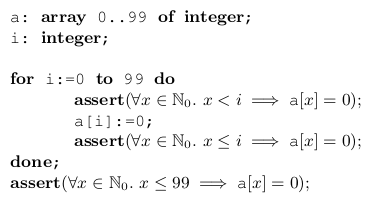
\includegraphics[scale=0.5]{code.png}\newline
$a[i]$ - array reading operator\newline
$a\{i\leftarrow x\}$ - array update operator\newline
$(\forall x \in \mathbb{N}_0. x < i \implies a[x] = 0) \wedge a' = a\{i\leftarrow 0\} \implies$\newline
$(\forall x \in \mathbb{N}_0. x \le i \implies a'[x] = 0)$
\end{frame}

\begin{frame}{Definitions}
\begin{itemize}
\item $T_I$ - index theory
\item $T_E$ - element theory
\item $T_A$ - array theory, $T_I \rightarrow T_E$
\end{itemize}
\begin{block}{Syntax}
$term A : array$-$identifier$ | term$_A\{$term$_I \leftarrow$ term$_E\}$\newline
$term E :$ term$_A[$term$_I]$ | $(previous rules)$\newline
$formula :$ term$_A$ = term$_A$ | $(previous rules)$\newline
\end{block}
\end{frame}

\begin{frame}{Definitions}
\begin{block}{Semantics}
\begin{itemize}
\item $\forall a_1 \in T_A. \forall a_2 \in T_A. \forall i \in T_I. \forall j \in T_I. (a_1 = a_2 \wedge i = j) \implies$\newline
$a_1[i] = a_2[j]$\newline
\item $\forall a \in T_A. \forall e \in T_E. \forall i \in T_I. \forall j \in T_I. a\{i\leftarrow e\}[j] = (i = j)? e : a[j]$\newline
\item$\forall a_1 \in T_A. \forall a_2 \in T_A. (\forall i \in T_I. a_1[i] = a_2 [i]) \implies$\newline
$a_1 = a_2$
\end{itemize}
\end{block}
\end{frame}

\begin{frame}{Eliminating the array terms}
We can therefore replace the array index operator by an uninterpreted function:\newline
$(i = j \wedge a[j] = 'z') \implies a[i] = 'z'$\newline
$(i = j \wedge F_a(i) = 'z') \implies F_a(i) = 'z'$\newline
\end{frame}

\begin{frame}{Write rule}
\begin{block}{Semantics}
\begin{itemize}
\item $a'[i] = e$ for the value that is written,
\item $\forall j \ne i. a'[j] = a[j]$ for the values that are unchanged.
\end{itemize}
\end{block}
$a[0] = 10 \implies a\{1 \leftarrow 20\}[0] = 10$\newline
\end{frame}

\begin{frame}{Write rule}
\begin{block}{Semantics}
\begin{itemize}
\item $a'[i] = e$ for the value that is written,
\item $\forall j \ne i. a'[j] = a[j]$ for the values that are unchanged.
\end{itemize}
\end{block}
$a[0] = 10 \implies a\{1 \leftarrow 20\}[0] = 10$\newline
$(a[0] = 10 \wedge a'[1] = 20 \wedge (\forall j \ne 1. a'[j] = a[j])) \implies a_0[0] = 10$\newline
$(F_a(0) = 10 \wedge F_{a'}(1) = 20 \wedge (\forall j \ne 1. F_{a'}(j) = F_a(j))) \implies F_{a'}(0) = 10$\newline
\end{frame}

\begin{frame}{Array property}
\begin{block}{}
An array theory formula is called an array property if and only if it is of the form\newline
$\forall i_1\dots \forall i_k \in T_I.\phi I (i_1, \dots, i_k) \Rightarrow \phi_V(i_1, \dots, i_k)$\newline
and satisfies the following conditions:
\begin{itemize}
\item The predicate $\phi$ , called the index guard, must follow the grammar\newline
$iguard : iguard \wedge iguard$ | $iguard \vee iguard$ | $iterm \le iterm$ | $iterm = iterm$\newline
$iterm : i_1$ | $\dots$ | $i_k$ | $term$\newline
$term$ : $integer$-$constant$ | $integer$-$constant * index$-$identifier$ | $term + term$\newline
The $index$-$identifier$ used in $term$ must not be one of $i_1, \dots, i_k$
\item The index variables $i_1, \dots, i_k$ can only be used in array read expressions of the form $a[i_j]$
\end{itemize}
The predicate $\phi_V$ is called the value constraint
\end{block}
\end{frame}

\begin{frame}{Example}
$a' = a\{i\leftarrow 0\}$\newline
\end{frame}

\begin{frame}{Example}
$a' = a\{i\leftarrow 0\}$\newline
$\forall j \ne i. a'[j] = a[j]$\newline
\end{frame}

\begin{frame}{Example}
$a' = a\{i\leftarrow 0\}$\newline
$\forall j \ne i. a'[j] = a[j]$\newline
$\forall j. (j \le i - 1 \wedge i + 1 \le j) \implies a'[j] = a[j]$
\end{frame}

\begin{frame}{$\iota(\phi)$}
\begin{block}{}
\begin{itemize}
\item All expressions used as an array index in $\phi$ that are not quantified variables
\item All expressions used inside index guards in $\phi$ that are not quantified variables
\item If $\phi$ contains none of the above, $\iota(\phi)$ is $\{0\}$ in order to obtain a nonempty set of index expressions
\end{itemize}
\end{block}
\end{frame}

\begin{frame}{Array reduction}
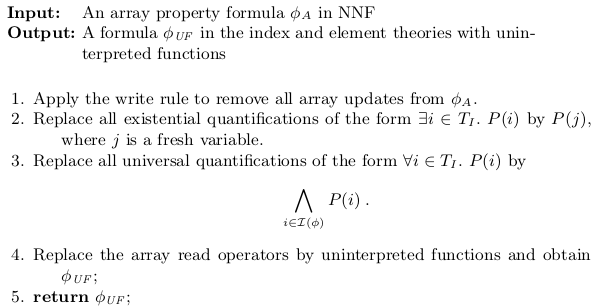
\includegraphics[scale=0.5]{array-reduction.png}
\end{frame}

\begin{frame}{Example}
$(\forall x \in \mathbb{N}_0. x < i \implies a[x] = 0) \wedge a' = a\{i\leftarrow 0\} \implies$\newline
$(\forall x \in \mathbb{N}_0. x \le i \implies a'[x] = 0)$
\end{frame}

\begin{frame}{Example}
$(\forall x \in \mathbb{N}_0. x < i \implies a[x] = 0) \wedge a' = a\{i\leftarrow 0\} \implies$\newline
$(\exists x \in \mathbb{N}_0. x \le i \wedge a'[x] \ne 0)$
\end{frame}

\begin{frame}{Example}
$(\forall x \in \mathbb{N}_0. x < i \implies a[x] = 0) \wedge a'[i] = 0 \wedge \forall j \ne i. a'[j] = a[j] \implies$\newline
$(\exists x \in \mathbb{N}_0. x \le i \wedge a'[x] \ne 0)$
\end{frame}

\begin{frame}{Example}
$(\forall x \in \mathbb{N}_0. x < i \implies a[x] = 0) \wedge a'[i] = 0 \wedge \forall j \ne i. a'[j] = a[j] \implies$\newline
$(z \le i \wedge a'[z] \ne 0)$
\end{frame}

\begin{frame}{Example}
$\iota(\phi) = \{i, z\}$
\end{frame}

\begin{frame}{Example}
$\iota(\phi) = \{i, z\}$\newline
$(i < i \implies a[i] = 0) \wedge (z < i \implies a[z] = 0) \wedge$\newline
$a'[i] = 0 \wedge \forall j \ne i. a'[j] = a[j] \implies$\newline
$(z \le i \wedge a'[z] \ne 0)$
\end{frame}

\begin{frame}{Example}
$\iota(\phi) = \{i, z\}$\newline
$(i < i \implies a[i] = 0) \wedge (z < i \implies a[z] = 0) \wedge$\newline
$a'[i] = 0 \wedge (i \ne i \implies a'[i] = a[i]) \wedge (z \ne i \implies a'[z] = a[z])\implies$\newline
$(z \le i \wedge a'[z] \ne 0)$
\end{frame}

\begin{frame}{Example}
$(z < i \implies a[z] = 0) \wedge$\newline
$a'[i] = 0 \wedge (z \ne i \implies a'[z] = a[z])\implies$\newline
$(z \le i \wedge a'[z] \ne 0)$
\end{frame}

\begin{frame}{Example}
$(z < i \implies F_a(z) = 0) \wedge$\newline
$F_{a'}(i) = 0 \wedge (z \ne i \implies F_{a'}(z) = F_a(z))\implies$\newline
$(z \le i \wedge F_{a'}(z) \ne 0)$
\end{frame}

\begin{frame}{Example}
$(z < i \implies F_a(z) = 0) \wedge$\newline
$F_{a'}(i) = 0 \wedge (z \ne i \implies F_{a'}(z) = F_a(z))\implies$\newline
$(z \le i \wedge F_{a'}(z) \ne 0)$\newline
\end{frame}

\begin{frame}{Example}
$(z < i \implies F_a(z) = 0) \wedge$\newline
$F_{a'}(i) = 0 \wedge (z \ne i \implies F_{a'}(z) = F_a(z))\implies$\newline
$(z \le i \wedge F_{a'}(z) \ne 0)$\newline
By distinguishing the three cases $z < i$, $z = i$, and $z > i$, it is easy to see that this formula is unsatisfiable
\end{frame}

\begin{frame}
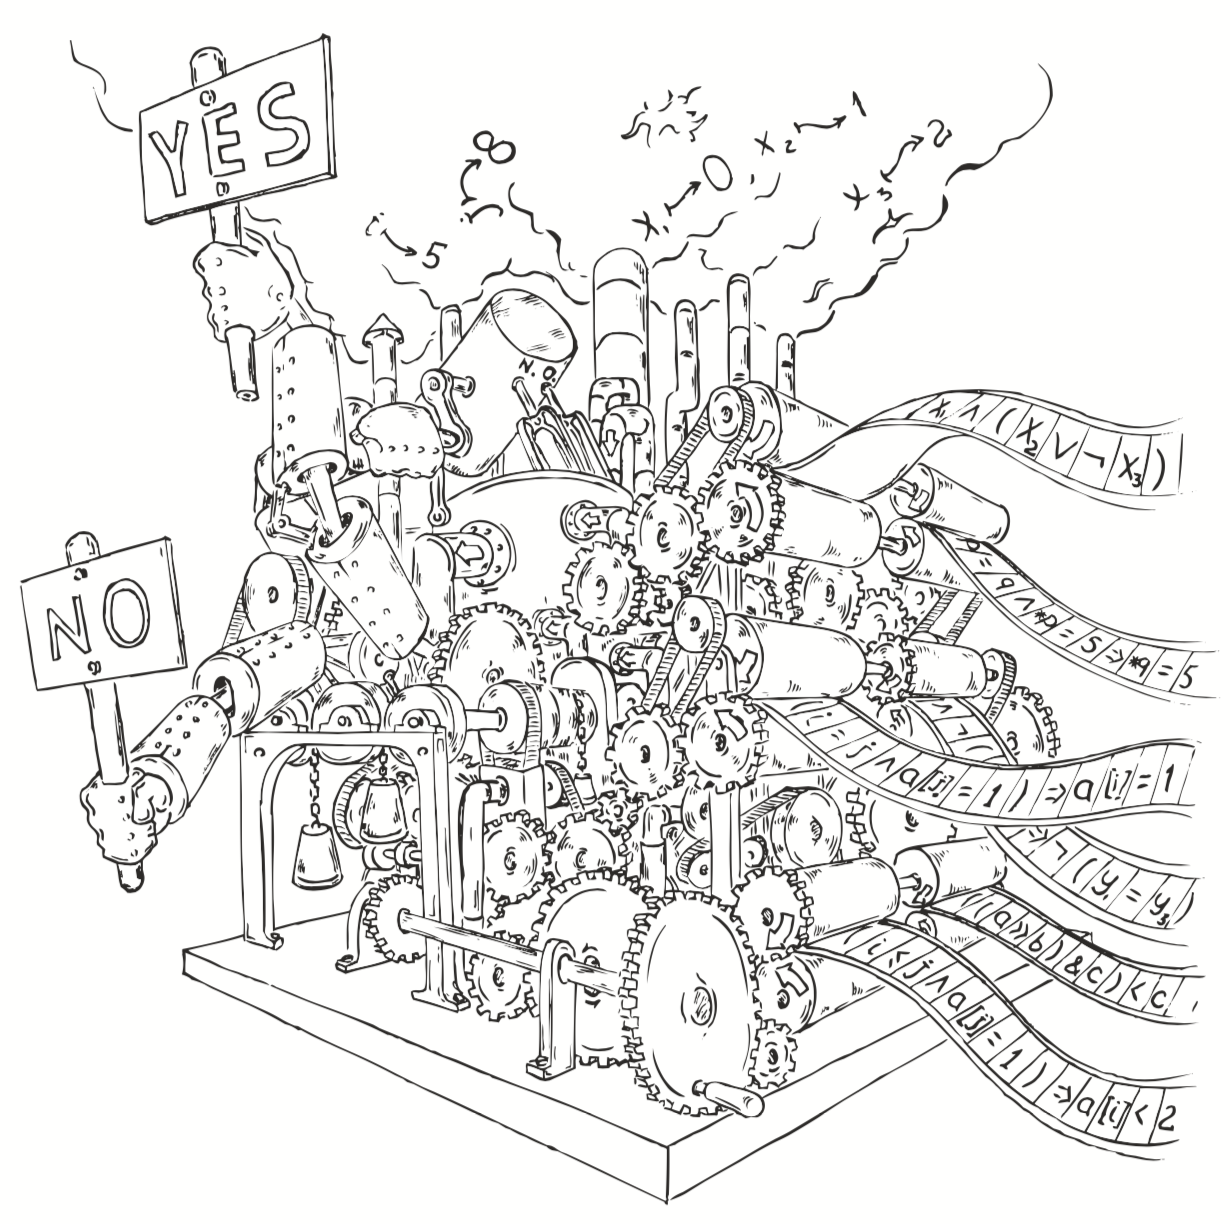
\includegraphics[scale=0.5]{../decision-procedure.png}
\end{frame}

\end{document}
